\chapter{معماری پیشنهادی: \lr{DuoDiT}}
\label{ch:proposed_method}

در این فصل، معماری پیشنهادی این پژوهش با عنوان \lr{DuoDiT} معرفی می‌شود. هدف این معماری، تنظیم دقیق پارامتر-کارای مدل‌های انتشار مبتنی بر مبدل (\lr{DiT}) برای کلاس‌ها یا دامنه‌های هدف است؛ به گونه‌ای که بدون به‌روزرسانی کامل بدنه اصلی، مسیر جداگانه‌ای برای استخراج و تزریق ویژگی‌های محلی فراهم شود. چالش اصلی در این مسئله آن است که تنظیم دقیق کامل مدل‌های بزرگ هزینه محاسباتی و حافظه‌ای بالایی دارد و در عین حال، روش‌های بسیار فشرده ممکن است برای تغییر بازنمایی‌های مکانی و حفظ جزئیات محلی کافی نباشند \cite{2212.09748,8409325}.

معماری \lr{DuoDiT} بر یک ساختار دوجریانی (\lr{Dual-Stream Architecture}) استوار است. جریان نخست، بدنه اصلی \lr{DiT} است که وزن‌های آن ثابت نگه داشته می‌شود و نقش حفظ دانش پیش‌آموزش‌دیده و ساختار معنایی تصویر را بر عهده دارد. جریان دوم، شاخه وضوح‌بالا یا شاخه \lr{x2} است که با اندازه پچ کوچک‌تر عمل می‌کند و ویژگی‌های ریزدانه‌تری تولید می‌کند. روش اصلی این پژوهش برای هم‌تراز کردن خروجی شاخه \lr{x2} با توکن‌های بدنه اصلی، مکانیزم «توکن‌های کلاس محلی» است؛ به این معنا که برای هر گروه محلی از چهار توکن وضوح‌بالا، یک توکن خلاصه‌ساز یادگیرنده تولید می‌شود و خروجی همین توکن به‌عنوان نماینده آن ناحیه به جریان اصلی افزوده می‌گردد \cite{2212.09748,chen2021crossvit,Dosovitskiy2020}.

\section{معماری مدل}
سیستم پیشنهادی از دو بخش اصلی تشکیل شده است. بخش نخست، \textbf{جریان بدنه اصلی منجمد (\lr{Frozen Backbone})} است که همان مدل \lr{DiT-XL/2} بوده و وزن‌های آن، شامل تعبیه‌ساز پچ، بلوک‌های مبدل و لایه‌های شرط‌گذاری اصلی، ثابت نگه داشته می‌شوند. این جریان بازنمایی اصلی نویز ورودی، زمان و برچسب کلاس را تولید می‌کند. بخش دوم، \textbf{جریان وضوح‌بالا (\lr{x2 Stream})} است که شامل تعبیه‌ساز پچ با اندازه کوچک‌تر، بلوک مبدل شاخه کمکی، مکانیزم تجمیع مبتنی بر توکن کلاس محلی و پروجکشن‌های تطبیق ابعاد است. معماری از نظر طراحی امکان افزودن شرط‌گذاری \lr{FiLM} را نیز دارد، اما این مؤلفه در آموزش اصلی \lr{ImageNet-1K} فعال نشده است \cite{2212.09748,Dosovitskiy2020,perez2018film}.

در پیاده‌سازی نهایی این پژوهش، ادغام دو جریان به‌صورت جمع باقی‌مانده پس از آخرین بلوک مبدل بدنه اصلی انجام می‌شود؛ این همان تنظیمی است که در فصل آزمایش‌ها با نام \lr{x2\_final\_fuse} گزارش شده است. بنابراین، گزینه‌هایی مانند ادغام متناوب در چندین بلوک، بخشی از فضای طراحی محسوب می‌شوند اما روش اصلی گزارش‌شده در این پایان‌نامه ادغام نهایی است \cite{Vaswani2017,2212.09748}.

شکل \ref{fig:proposed_architecture_overview} نمای کلی جریان معماری پیشنهادی را نشان می‌دهد. در این نما، مسیر بدنه اصلی \lr{DiT} در کنار شاخه وضوح‌بالا قرار گرفته و نقش مکانیزم توکن‌های کلاس محلی در فشرده‌سازی و انتقال ویژگی‌های شاخه \lr{x2} به جریان اصلی مشخص شده است.

\begin{figure}[H]
    \centering
    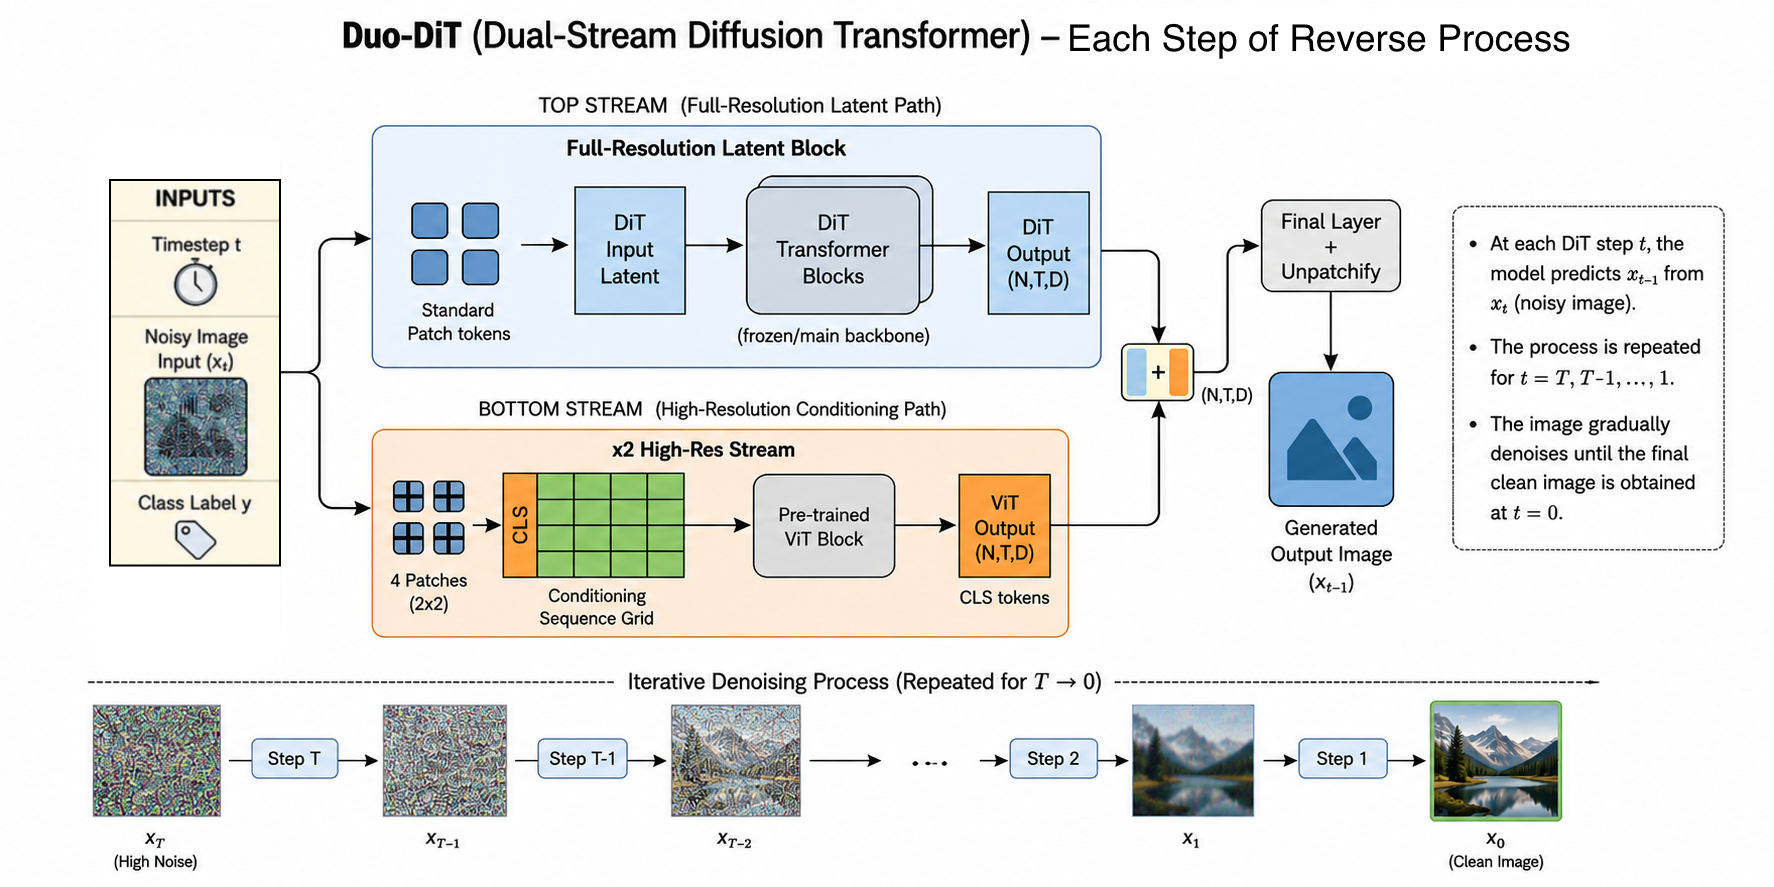
\includegraphics[width=0.95\linewidth]{images/duodit-arch-overview.drawio.png}
    \caption[نمای کلی معماری پیشنهادی مبتنی بر توکن‌های کلاس محلی]{نمای کلی معماری پیشنهادی و جریان تجمیع ویژگی مبتنی بر توکن‌های کلاس محلی. شاخه وضوح‌بالا ویژگی‌های ریزدانه را استخراج کرده و توکن‌های کلاس محلی، اطلاعات هر گروه از توکن‌ها را برای ادغام با بدنه اصلی \lr{DiT} فشرده می‌کنند.}
    \label{fig:proposed_architecture_overview}
\end{figure}

\subsection{تعبیه‌ساز پچ با وضوح بالا}
در مدل استاندارد \lr{DiT-XL/2}، ورودی نهان به پچ‌های $2 \times 2$ تقسیم می‌شود. در شاخه \lr{x2}، برای افزایش تفکیک مکانی اولیه، اندازه پچ برابر $p'=1$ در نظر گرفته شده است. اگر تعداد توکن‌های شاخه اصلی برابر $T$ باشد، شاخه \lr{x2} چهار برابر آن، یعنی $4T$ توکن تولید می‌کند. این اختلاف تعداد توکن‌ها باعث می‌شود پیش از ادغام با جریان اصلی، یک مرحله هم‌ترازسازی و کاهش طول توالی لازم باشد. روش اصلی این هم‌ترازسازی در این پژوهش، مکانیزم توکن کلاس محلی است \cite{2212.09748,Dosovitskiy2020}.

\subsection{روش‌های تجمیع ویژگی}
سه راهبرد ساده‌تر برای کاهش طول توالی شاخه \lr{x2} در نظر گرفته شده‌اند تا در فصل آزمایش‌ها با روش توکن کلاس محلی مقایسه شوند. این راهبردها بخشی از معماری نهایی نیستند، بلکه نقش مبناهای مقایسه‌ای را دارند \cite{726791,chen2021crossvit}.

\subsubsection{تجمیع با پروجکشن خطی}
در این روش، برای کاهش ابعاد و ادغام ویژگی‌های شاخه \lr{x2} با بدنه اصلی، از مکانیسم الحاق و پروجکشن خطی استفاده می‌شود. برای هر ناحیه $2 \times 2$ از تصویر که متناظر با ۴ توکن در شاخه با وضوح بالا است، ویژگی‌ها به صورت برداری به یکدیگر متصل می‌شوند \cite{2212.09748,chen2021crossvit}.
فرض کنید $Z_{x2}$ ویژگی‌های ورودی باشند. برای هر موقعیت $i$، چهار توکن $z_{4i}, z_{4i+1}, z_{4i+2}, z_{4i+3}$ وجود دارد. خروجی تجمیع شده $z'_i$ به صورت زیر محاسبه می‌شود:
\begin{equation}
    \label{eq:linear-projection-aggregation}
    z'_i = W \cdot \text{Concat}(z_{4i}, z_{4i+1}, z_{4i+2}, z_{4i+3}) + b
\end{equation}
\begin{figure}[H]
    \centering
    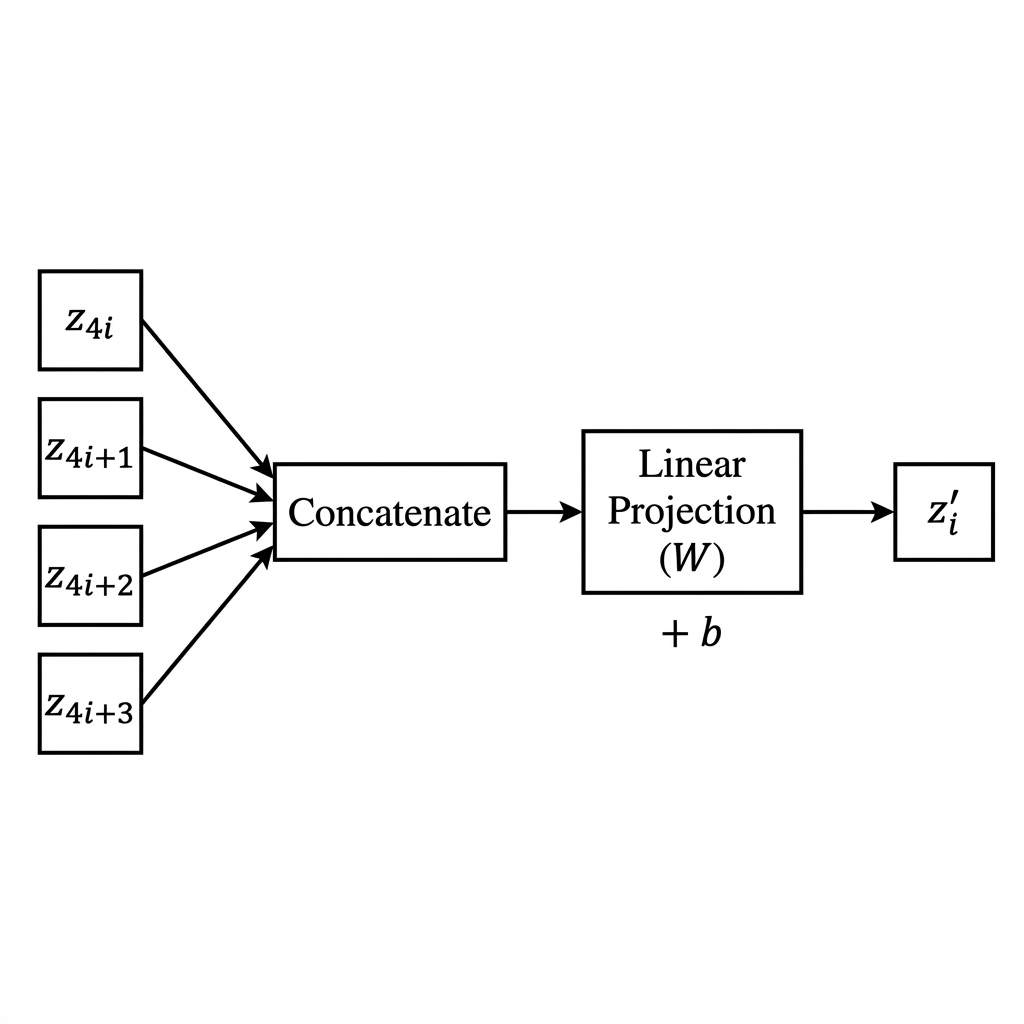
\includegraphics[width=0.9\linewidth]{images/linear_projection_aggregation.png}
    \caption[تجمیع ویژگی با پروجکشن خطی]{نمای شماتیک از تجمیع ویژگی با استراتژی پروجکشن خطی. انطباق ۴ توکن ورودی به یک توکن خروجی با استفاده از پروجکشن خطی.}
    \label{fig:linear_proj}
\end{figure}
در این رابطه، $W$ ماتریس وزن لایه خطی است که ابعاد فضای ویژگی ادغام شده را به ابعاد فضای هدف تطبیق می‌دهد. شکل \ref{fig:linear_proj} این نگاشت چهار توکن ورودی به یک توکن خروجی را به‌صورت شماتیک نشان می‌دهد.

\subsubsection{تجمیع با \lr{Max Pooling}}
در این رویکرد، برای استخراج ویژگی نهایی از هر پچ، از عملیات \lr{Max Pooling} استفاده می‌شود. این روش بر این فرض استوار است که بیشینه مقدار فعالیت در هر کانال ویژگی، بیانگر برجسته‌ترین اطلاعات آن ناحیه است \cite{726791}.
برای هر گروه ۴ تایی از توکن‌ها که مربوط به یک پچ از تصویر اصلی هستند، مقدار بیشینه در هر بعد ویژگی محاسبه می‌شود:
\begin{equation}
    \label{eq:max-pooling-aggregation}
    z'_{i,j} = \max(z_{4i,j}, z_{4i+1,j}, z_{4i+2,j}, z_{4i+3,j})
\end{equation}
در اینجا $z'_{i,j}$ مقدار $j$-امین ویژگی از $i$-امین توکن خروجی است. این عملیات بدون استفاده از پارامترهای یادگیرنده انجام می‌شود.

\subsubsection{تجمیع با \lr{Min Pooling}}
این روش مشابه رویکرد \lr{Max Pooling} است، با این تفاوت که از عملیات \lr{Min Pooling} استفاده می‌کند. در اینجا تمرکز بر کمینه مقدار سیگنال در هر زیر-ناحیه است.
رابطه ریاضی این تبدیل به صورت زیر تعریف می‌شود:
\begin{equation}
    \label{eq:min-pooling-aggregation}
    z'_{i,j} = \min(z_{4i,j}, z_{4i+1,j}, z_{4i+2,j}, z_{4i+3,j})
\end{equation}
\begin{figure}[H]
    \centering
    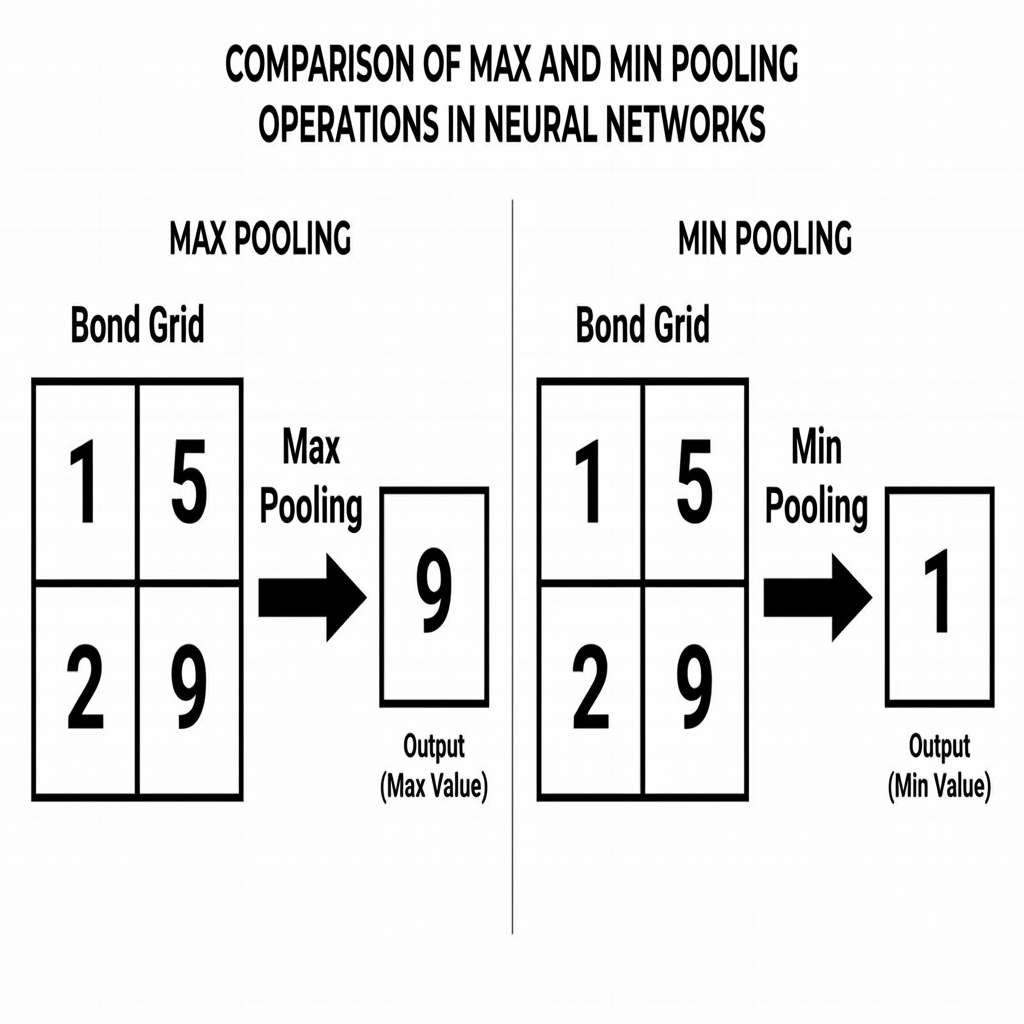
\includegraphics[width=0.9\linewidth]{images/pooling_operations.png}
    \caption[مقایسه \lr{Max Pooling} و \lr{Min Pooling}]{مقایسه عملیات \lr{Max Pooling} و \lr{Min Pooling}. در سمت چپ، انتخاب بیشینه مقدار و در سمت راست، انتخاب کمینه مقدار مشاهده می‌شود.}
    \label{fig:pooling_ops}
\end{figure}
این رویکرد نیز همانند روش بیشینه، یک عملیات ثابت و بدون وزن‌های قابل آموزش است که اطلاعات مکانی را با انتخاب اکسترمم‌ها فشرده‌سازی می‌کند. شکل \ref{fig:pooling_ops} تفاوت انتخاب بیشینه و کمینه را در این نوع تجمیع نشان می‌دهد.

\subsection{روش تجمیع ویژگی با توکن}
\label{sec:local_cls}
در معماری نهایی \lr{DuoDiT}، کاهش طول توالی شاخه \lr{x2} به‌صورت یک عملیات یادگیرنده انجام می‌شود. در روش‌های ثابت مانند میانگین‌گیری یا بیشینه‌گیری، قاعده فشرده‌سازی مستقل از محتوای تصویر است؛ در نتیجه، همه گروه‌های محلی با یک قانون یکسان خلاصه می‌شوند. در مقابل، توکن کلاس محلی یک بردار یادگیرنده است که همراه با توکن‌های هر ناحیه پردازش می‌شود و می‌تواند بر اساس الگوی محلی همان ناحیه، بازنمایی فشرده‌تری تولید کند \cite{726791,Dosovitskiy2020,chen2021crossvit}.

در مدل‌های استاندارد \lr{ViT}، یک توکن کلاس سراسری برای خلاصه‌سازی کل تصویر به کار می‌رود. در این پژوهش، همین ایده در مقیاس محلی استفاده شده است: هر چهار توکن شاخه \lr{x2} که متناظر با یک توکن شاخه اصلی هستند، همراه با یک توکن کلاس محلی وارد بلوک پردازشی می‌شوند و خروجی توکن کلاس به عنوان نماینده همان ناحیه انتخاب می‌شود. بنابراین، خروجی شاخه \lr{x2} از $4T$ توکن به $T$ توکن کاهش می‌یابد و از نظر طول توالی با بدنه اصلی هم‌راستا می‌شود. شکل \ref{fig:local_cls} سازوکار گروه‌بندی توکن‌ها و استخراج خروجی محلی را نمایش می‌دهد \cite{Dosovitskiy2020,chen2021crossvit}.

\begin{figure}[H]
    \centering
    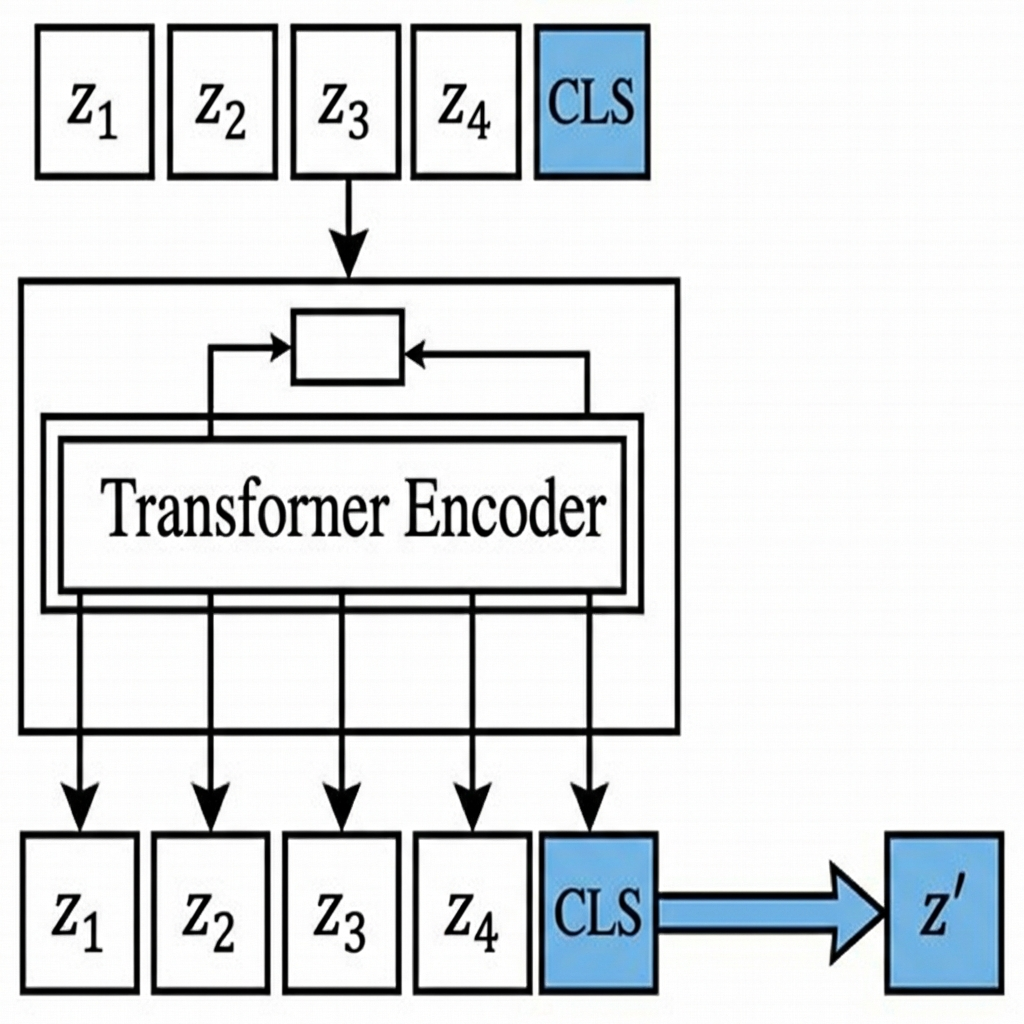
\includegraphics[width=0.9\linewidth]{images/local_cls_mechanism.png}
    \caption[مکانیزم توکن کلاس محلی]{نمای شماتیک از مکانیزم توکن کلاس محلی. توکن‌های داده در گروه‌های ۴تایی به همراه یک توکن کلاس یادگیرنده وارد بلوک پردازشی شده و تنها توکن کلاس به عنوان خروجی انتخاب می‌شود.}
    \label{fig:local_cls}
\end{figure}

فرآیند عملیاتی این روش شامل سه مرحله است. فرض کنید خروجی تعبیه‌ساز شاخه وضوح‌بالا با $Z_{x2} \in \mathbb{R}^{N \times 4T \times D}$ نمایش داده شود، که در آن $N$ اندازه دسته، $4T$ طول توالی شاخه \lr{x2} و $D$ بعد ویژگی است. در گام نخست، توکن‌ها بر اساس موقعیت مکانی به گروه‌های چهارتایی تقسیم می‌شوند:
\begin{equation}
    \label{eq:local-cls-grouping}
    Z_{\text{grouped}} = \text{Reshape}(Z_{x2}) \in \mathbb{R}^{N \times T \times 4 \times D}
\end{equation}
در این مرحله، $T$ گروه مجزا وجود دارد که هر گروه شامل چهار بردار ویژگی $z_{4i}, z_{4i+1}, z_{4i+2}, z_{4i+3}$ است.

در گام دوم، یک پارامتر قابل یادگیری اولیه $C_{init} \in \mathbb{R}^{1 \times 1 \times D}$ تعریف می‌شود و برای تمام گروه‌ها و تمام نمونه‌های دسته گسترش می‌یابد. سپس این توکن به انتهای هر گروه چهارتایی الحاق می‌شود و ورودی محلی پنج‌توکنی شکل می‌گیرد:
\begin{equation}
    \label{eq:local-cls-input}
    Z_{\text{input}}^{(i)} = \text{Concat}([z_{4i}, \dots, z_{4i+3}, c_{\text{token}}^{(i)}]) \in \mathbb{R}^{5 \times D}
\end{equation}
که در آن $Z_{\text{input}}^{(i)}$ ورودی مربوط به $i$-امین پنجره محلی است.

در گام سوم، گروه‌های پنج‌تایی به صورت توالی $N \times 5T \times D$ بازآرایی می‌شوند و از بلوک مبدل شاخه \lr{x2} عبور می‌کنند. در پیاده‌سازی نهایی، محلی بودن تجمیع از طریق گروه‌بندی چهارتایی و استخراج خروجی توکن کلاس هر گروه اعمال می‌شود؛ به بیان دیگر، پس از پردازش، فقط موقعیت‌های متناظر با توکن‌های کلاس نگه داشته می‌شوند:
\begin{equation}
    \label{eq:local-cls-transformer}
    Z_{\text{processed}} = \text{TransformerEncoder}(Z_{\text{flattened}})
\end{equation}
خروجی این تبدیل نیز دارای ابعاد $N \times 5T \times D$ است. وزن‌های بلوک مبدل و توکن کلاس محلی در طول آموزش تنظیم می‌شوند تا خروجی توکن کلاس بتواند بازنمایی فشرده‌ای از همان گروه محلی ایجاد کند.

در گام نهایی، از میان پنج خروجی مربوط به هر گروه، فقط بردار خروجی موقعیت توکن کلاس انتخاب می‌شود:
\begin{equation}
    \label{eq:local-cls-extraction}
    z'_{i} = Z_{\text{processed}}[i \times 5 + 4]
\end{equation}
(با فرض اینکه توکن کلاس در اندیس آخر، یعنی اندیس ۴ الحاق شده باشد).
بدین ترتیب، خروجی نهایی شاخه کمکی با $Z_{\text{cls}} \in \mathbb{R}^{N \times T \times D}$ نمایش داده می‌شود و از نظر طول توالی با خروجی بدنه اصلی سازگار است.

\subsection{مبدل بینایی به عنوان خبره (\lr{ViT as Expert})}
برای پردازش ویژگی‌های شاخه \lr{x2}، از یک بلوک مبدل برگرفته از مدل \lr{vit\_large\_patch16\_224} استفاده شده است. این بلوک با وزن‌های پیش‌آموزش‌دیده مقداردهی اولیه می‌شود تا شاخه کمکی از ابتدا دارای بازنمایی‌های بصری قابل استفاده باشد. از آنجا که بعد پنهان این مدل \lr{ViT} با بعد پنهان \lr{DiT-XL/2} یکسان نیست، پروجکشن‌های خطی ورودی و خروجی برای تبدیل ابعاد استفاده می‌شوند \cite{Dosovitskiy2020,5206848,2212.09748,wightman2019timm}.

\subsection{شرط‌گذاری اختیاری با \lr{FiLM}}
معماری \lr{DuoDiT} از نظر طراحی می‌تواند شاخه \lr{x2} را با مدولاسیون خطی ویژگی (\lr{FiLM}) به گام زمانی نویز و برچسب کلاس وابسته کند، اما این گزینه در آموزش اصلی \lr{ImageNet-1K} این پایان‌نامه فعال نشده است. بنابراین، نتایج فصل آزمایش‌ها بر اساس ویژگی‌های بدون مدولاسیون شاخه دوم گزارش می‌شوند و \lr{FiLM} به عنوان یک مسیر توسعه اختیاری برای تنظیمات شرطی پیچیده‌تر باقی می‌ماند \cite{perez2018film,2088740}.

در حالت فعال، بردار شرط $c = e_t + e_y$، که از ترکیب تعبیه زمان و تعبیه کلاس به دست می‌آید، به یک شبکه \lr{MLP} داده می‌شود تا ضرایب مقیاس و انتقال تولید شوند. این ضرایب پیش از ورود ویژگی‌های شاخه \lr{x2} به بلوک مبدل اعمال می‌شوند:
\begin{equation}
    \label{eq:film-conditioning}
    x_2' = \gamma(c) \cdot x_2 + \beta(c)
\end{equation}
\begin{figure}[H]
    \centering
    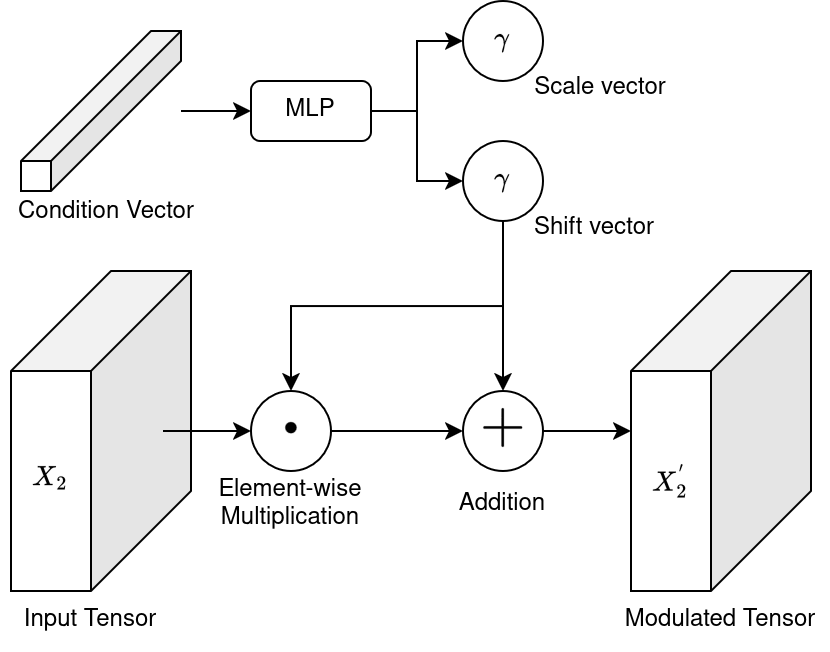
\includegraphics[width=0.9\linewidth]{images/film_modulation.png}
    \caption[بلوک شرط‌گذاری \lr{FiLM}]{بلوک شرط‌گذاری \lr{FiLM}. بردار شرط $c$ پارامترهای مقیاس و انتقال را تولید می‌کند که بر روی ورودی اعمال می‌شوند.}
    \label{fig:film_mod}
\end{figure}
سازوکار تولید و اعمال ضرایب مقیاس و انتقال در شکل \ref{fig:film_mod} نشان داده شده است. بررسی اثر فعال‌سازی این ماژول در رژیم‌های شرطی ریزدانه‌تر می‌تواند به عنوان یکی از مسیرهای آینده دنبال شود.

\subsection{ادغام نهایی}
پس از استخراج توکن‌های کلاس محلی، خروجی شاخه \lr{x2} از نظر طول توالی با خروجی بدنه اصلی هم‌اندازه است. در معماری نهایی این پژوهش، ادغام فقط در انتهای بدنه اصلی انجام می‌شود. اگر خروجی آخرین بلوک بدنه اصلی با $H_{\text{backbone}}^{(L)}$ و خروجی هم‌تراز شاخه کمکی با $H_{x2}$ نمایش داده شود، اتصال باقی‌مانده نهایی به صورت زیر است:
\begin{equation}
    \label{eq:dual-stream-fusion}
    H_{\text{fused}} = H_{\text{backbone}}^{(L)} + H_{x2}
\end{equation}
سپس 
$H_{\text{fused}}$
 وارد لایه نهایی 
 \lr{DiT}
 تا ویژگی‌های نهایی به دست آیند.
 
\section{استراتژی آموزش و تنظیم دقیق}
استراتژی آموزش \lr{DuoDiT} بر ثابت نگه داشتن بدنه اصلی و آموزش اجزای شاخه کمکی مبتنی است. هدف این طراحی، کاهش تعداد پارامترهای به‌روزرسانی‌شونده در عین حفظ امکان سازگارسازی بازنمایی‌های محلی است \cite{8409325,2212.09748}.

\subsection{مدیریت پارامترهای منجمد و آموزش‌پذیر}
در این روش، بدنه اصلی مدل انتشار (\lr{DiT Backbone}) که شامل لایه‌های تعبیه ورودی، بلوک‌های مبدل اصلی و لایه‌های مدولاسیون است، به طور کامل \textbf{منجمد (\lr{Frozen})} نگه داشته می‌شود. این کار باعث می‌شود دانش پیش‌آموزش‌دیده مدل پایه در طول تنظیم دقیق تغییر نکند \cite{8409325,2212.09748}.
در مقابل، اجزای زیر به عنوان پارامترهای قابل آموزش (\lr{Trainable Parameters}) فعال می‌شوند:
\begin{itemize}
    \item \textbf{تعبیه‌ساز پچ شاخه \lr{x2}}: برای یادگیری بازنمایی‌های اولیه با وضوح بالا.
    \item \textbf{توکن‌های کلاس محلی}: پارامترهای یادگیرنده‌ای که بازنمایی هر گروه محلی را خلاصه می‌کنند.
    \item \textbf{بلوک مبدل شاخه \lr{x2} و پروجکشن‌ها}: جهت پردازش عمیق ویژگی‌های جزئیات.
    \item \textbf{لایه خروجی (\lr{Final Layer})}: که امکان تطبیق نهایی خروجی مدل با فضای هدف را فراهم می‌کند.
\end{itemize}
این تفکیک پارامترها باعث می‌شود تنها \lr{17.95} میلیون پارامتر از مجموع \lr{690.39} میلیون پارامتر نیازمند ذخیره گرادیان و به‌روزرسانی باشند.

\subsection{مقداردهی اولیه با وزن‌های پیش‌آموزش‌دیده}
برای مقداردهی اولیه بلوک مبدل شاخه \lr{x2}، از وزن‌های پیش‌آموزش‌دیده مدل \lr{ViT-Large} آموزش‌دیده روی \lr{ImageNet} استفاده می‌شود. در صورتی که ابعاد فضای پنهان مدل \lr{DiT} با ابعاد مدل \lr{ViT} بارگذاری‌شده تفاوت داشته باشد، لایه‌های پروجکشن خطی برای تطبیق ابعاد اضافه و آموزش داده می‌شوند \cite{Dosovitskiy2020,5206848,wightman2019timm,2212.09748}.

\subsection{تثبیت آموزش با \lr{EMA}}
برای پایداری فرآیند آموزش و جلوگیری از نوسانات شدید در وزن‌ها، از روش میانگین متحرک نمایی\LTRfootnote{Exponential Moving Average} (\lr{EMA}) استفاده می‌شود. یک نسخه کپی از مدل که وزن‌های آن میانگین متحرک وزن‌های در حال آموزش است، نگهداری می‌شود و در نهایت برای تولید نمونه‌ها و ارزیابی کیفیت مورد استفاده قرار می‌گیرد \cite{2212.09748}.

\subsection{الگوریتم آموزش}
الگوریتم \ref{alg:training} روند آموزش \lr{DuoDiT} را به صورت گام‌به‌گام نشان می‌دهد. در این الگوریتم، بدنه اصلی \lr{DiT} ثابت است، شاخه \lr{x2} با توکن‌های کلاس محلی آموزش داده می‌شود، و ادغام دو جریان پس از آخرین بلوک بدنه اصلی انجام می‌گیرد.

برای پشتیبانی از \lr{CFG} در مرحله نمونه‌برداری، آموزش فقط به حالت شرطی محدود نمی‌شود. در هر تکرار، برچسب کلاس با احتمال $p_{\text{\lr{drop}}}$ با شرط تهی جایگزین می‌شود تا مدل واحد بتواند هر دو پیش‌بینی شرطی و بی‌شرط را یاد بگیرد. این کار تغییری در معماری \lr{DuoDiT} ایجاد نمی‌کند، اما در زمان نمونه‌برداری امکان ترکیب دو خروجی
$\epsilon_\theta(x_t,t,y)$
و
$\epsilon_\theta(x_t,t,\emptyset)$
را با ضریب \lr{CFG} فراهم می‌سازد \cite{ho2022classifierFreeGuidance}.

\begin{latin}
\begin{algorithm}[htbp]
\caption{Parameter-Efficient Training Loop for DuoDiT}
\label{alg:training}
\begin{algorithmic}[1]
\Require Pre-trained DiT Backbone $\theta_{\text{frozen}}$, Trainable x2-stream parameters $\phi$, Dataset $\mathcal{D}$, Learning Rate $\eta$, Label-drop probability $p_{\text{drop}}$
\State Initialize Second Stream Expert ViT block with pre-trained weights
\State Freeze all parameters in $\theta_{\text{frozen}}$
\While{not converged}
    \State Sample batch of images $x_0 \sim \mathcal{D}$ and class labels $y$
    \State With probability $p_{\text{drop}}$, replace $y$ with the null condition $\emptyset$
    \State Sample time steps $t \sim \text{Uniform}(1, T)$
    \State Sample noise $\epsilon \sim \mathcal{N}(0, I)$
    \State Compute noisy image $x_t = \sqrt{\bar{\alpha}_t}x_0 + \sqrt{1 - \bar{\alpha}_t}\epsilon$
    \State Extract final frozen-backbone features $h_{\text{backbone}}^{(L)} = \mathcal{F}(x_t, t, y; \theta_{\text{frozen}})$
    \State Extract high-resolution x2 tokens $h_{x2} = \mathcal{E}_{x2}(x_t; \phi_{\text{embed}})$
    \State Use (modulated) Second Stream features $h_{x2}' = h_{x2}$
    \State Group x2 tokens in sets of four and append local class tokens
    \State Process grouped sequence through Expert ViT block
    \State Extract local class-token positions and project them to DiT hidden dimension: $h_{\text{cls}}$
    \State Fuse after the final backbone block: $h_{\text{fused}} = h_{\text{backbone}}^{(L)} + h_{\text{cls}}$
    \State Predict noise $\epsilon_\theta = \text{FinalLayer}(h_{\text{fused}}; \phi_{\text{out}})$
    \State Compute Loss $\mathcal{L} = \| \epsilon - \epsilon_\theta \|^2$
    \State Update $\phi \gets \phi - \eta \nabla_\phi \mathcal{L}$
    \State Update EMA parameters $\phi_{\text{ema}} \gets 0.9999 \phi_{\text{ema}} + 0.0001 \phi$
\EndWhile
\end{algorithmic}
\end{algorithm}
\end{latin}

\subsection{کارایی پارامتری}
جدول \ref{tab:param_count} تحلیل کلان تعداد پارامترهای قابل آموزش در معماری \lr{DuoDiT} را نشان می‌دهد. با منجمد نگه‌داشتن بدنه اصلی \lr{DiT-XL/2} و آموزش فقط شاخه دوم، توکن‌های کلاس محلی، پروجکشن‌ها و لایه خروجی، تعداد پارامترهای آموزش‌پذیر به \lr{17.95} میلیون از \lr{690.39} میلیون پارامتر کل محدود می‌شود. این کاهش در تعداد وزن‌های به‌روزرسانی‌شونده، امکان اجرای تنظیم دقیق پارامتر-کارا را با هزینه حافظه و زمان کمتر فراهم می‌کند \cite{2212.09748,8409325}.

\begin{table}[htbp]
    \centering
    \caption[تحلیل پیچیدگی مدل]{تحلیل پیچیدگی مدل و تفکیک پارامترهای قابل آموزش}
    \label{tab:param_count}
    \begin{latin}
    \begin{tabular}{lrc}
        \hline
        \textbf{Component} & \textbf{Parameters (M)} & \textbf{Trainable} \\
        \hline
        Frozen DiT-XL/2 Backbone & 672.44 & False \\
        Trainable DuoDiT Components & 17.95 & True \\
        \hline
        \textbf{Total Parameters} & \textbf{690.39} & \\
        \hline
    \end{tabular}
    \end{latin}
\end{table}

\section{تابع هزینه}
فرض کنید $x_t$ نمونه نویزی در گام زمانی $t$ و $y$ برچسب کلاس باشد. بدنه اصلی منجمد با پارامترهای $\theta$ خروجی آخرین بلوک خود را به صورت زیر تولید می‌کند \cite{6206256,2212.09748}:
\begin{equation}
    \label{eq:backbone-final}
    H_{\text{backbone}}^{(L)} = \mathcal{F}_{\theta}(x_t, t, y), \quad
    H_{\text{backbone}}^{(L)} \in \mathbb{R}^{N \times T \times D}.
\end{equation}
شاخه \lr{x2} همان ورودی نویزی را با اندازه پچ کوچک‌تر پردازش می‌کند و توالی بلندتری به دست می‌دهد:
\begin{equation}
    \label{eq:x2-embed}
    Z_{x2} = \mathcal{E}_{x2}(x_t), \quad
    Z_{x2} \in \mathbb{R}^{N \times 4T \times D}.
\end{equation}
در آموزش اصلی این پژوهش، شاخه کمکی بدون مدولاسیون \lr{FiLM} وارد مرحله تجمیع می‌شود:
\begin{equation}
    \label{eq:x2-film}
    \tilde{Z}_{x2} = Z_{x2}.
\end{equation}
توکن‌های شاخه کمکی مطابق رابطه \ref{eq:local-cls-grouping} در گروه‌های چهارتایی قرار می‌گیرند، توکن کلاس محلی به هر گروه افزوده می‌شود و توالی حاصل از بلوک مبدل شاخه کمکی عبور می‌کند:
\begin{equation}
    \label{eq:x2-expert}
    U = \mathcal{T}_{\phi}(\text{Flatten}([\text{Group}(\tilde{Z}_{x2}); C])),
    \quad U \in \mathbb{R}^{N \times 5T \times D}.
\end{equation}
با انتخاب خروجی‌های متناظر با توکن‌های کلاس، توالی شاخه کمکی به طول $T$ کاهش می‌یابد:
\begin{equation}
    \label{eq:x2-cls-sequence}
    H_{x2} = \text{SelectClassToken}(U), \quad
    H_{x2} \in \mathbb{R}^{N \times T \times D}.
\end{equation}
در نهایت، خروجی شاخه کمکی پس از هم‌ترازسازی ابعاد، به خروجی آخرین بلوک بدنه اصلی افزوده می‌شود و لایه نهایی نویز را پیش‌بینی می‌کند:
\begin{equation}
    \label{eq:duodit-output}
    \epsilon_{\theta,\phi}(x_t,t,y) =
    \text{FinalLayer}_{\phi}(H_{\text{backbone}}^{(L)} + H_{x2}).
\end{equation}
تابع هزینه آموزشی همان خطای رایج پیش‌بینی نویز در مدل‌های انتشار است \cite{6206256,2212.09748}:
\begin{equation}
    \label{eq:duodit-loss}
    \mathcal{L}_{\text{DuoDiT}} =
    \mathbb{E}_{x_0,t,\epsilon,y}
    \left[
    \left\|
    \epsilon - \epsilon_{\theta,\phi}(x_t,t,y)
    \right\|_2^2
    \right].
\end{equation}
در این رابطه‌ها، $\theta$ ثابت است و فقط پارامترهای $\phi$، شامل تعبیه‌ساز شاخه \lr{x2}، توکن‌های کلاس محلی، بلوک مبدل شاخه کمکی، پروجکشن‌ها و لایه نهایی، به‌روزرسانی می‌شوند.

\section{جمع‌بندی}
در این فصل، معماری \lr{DuoDiT} برای تنظیم دقیق پارامتر-کارای مدل \lr{DiT} معرفی شد. روش نهایی شامل یک بدنه اصلی منجمد و یک شاخه وضوح‌بالا است که خروجی آن با مکانیزم توکن کلاس محلی از $4T$ توکن به $T$ توکن کاهش می‌یابد. سپس خروجی هم‌تراز شاخه کمکی پس از آخرین بلوک بدنه اصلی با جریان اصلی جمع شده و وارد لایه نهایی می‌شود. در این ساختار، راهبردهای ساده‌تری مانند پروجکشن خطی، بیشینه‌گیری و کمینه‌گیری به عنوان مبناهای مقایسه‌ای در نظر گرفته شده‌اند، اما معماری اصلی گزارش‌شده در این پایان‌نامه بر تجمیع مبتنی بر توکن کلاس محلی و ادغام نهایی \lr{x2\_final\_fuse} متکی است.
